\documentclass[11pt,a4paper]{article}

\usepackage[utf8]{inputenc}
\usepackage[T1]{fontenc}
\usepackage[margin=2.2cm]{geometry}
\usepackage{parskip}
\usepackage{titlesec}
\usepackage{enumitem}
\usepackage{booktabs}
\usepackage{xcolor}
\usepackage{tcolorbox}
\usepackage{graphicx}
\usepackage{hyperref}
\usepackage{fancyhdr}
\usepackage{listings}
\usepackage{longtable}
\usepackage{array}

\tcbuselibrary{skins,breakable}

\renewcommand{\contentsname}{Contenido}
\renewcommand{\figurename}{Figura}
\renewcommand{\tablename}{Tabla}

\definecolor{accent}{RGB}{30,80,150}
\definecolor{softgray}{RGB}{245,246,248}
\definecolor{codebg}{RGB}{248,248,250}
\definecolor{warn}{RGB}{160,60,40}
\definecolor{good}{RGB}{30,120,70}

\titleformat{\section}{\Large\bfseries\color{accent}}{\thesection}{0.8em}{}
\titleformat{\subsection}{\large\bfseries}{\thesubsection}{0.6em}{}
\titleformat{\subsubsection}{\normalsize\bfseries\itshape}{\thesubsubsection}{0.5em}{}

\hypersetup{
  colorlinks=true, linkcolor=accent, urlcolor=accent,
  pdftitle={AgentIA --- Revisión del sistema, verificación y coste},
  pdfauthor={Ingeniería AgentIA}
}

\pagestyle{fancy}
\fancyhf{}
\fancyhead[L]{\small\color{accent}AgentIA --- Revisión del sistema}
\fancyhead[R]{\small\color{accent}\thepage}
\renewcommand{\headrulewidth}{0.4pt}

\lstset{
  basicstyle=\ttfamily\small, backgroundcolor=\color{codebg},
  frame=single, rulecolor=\color{softgray}, breaklines=true,
  columns=fullflexible, keepspaces=true, showstringspaces=false,
  xleftmargin=0.5em, xrightmargin=0.5em,
}

\newtcolorbox{notebox}[1][]{colback=softgray,colframe=accent,boxrule=0.4pt,
  arc=2pt,left=6pt,right=6pt,top=4pt,bottom=4pt,breakable,#1}

\title{\vspace{-1.4cm}\textbf{AgentIA --- Revisión del sistema, verificación y coste}\\[0.25cm]
\large El flujo de trabajo agéntico, la orquestación, lo que se mide y lo que cuesta}
\author{Ingeniería AgentIA}
\date{2026-09-29}

\begin{document}
\maketitle
\thispagestyle{fancy}

\begin{notebox}
\textbf{Qué es este documento.} Una revisión del sistema tal como se ejecuta hoy: el
flujo de trabajo agéntico de generación (el pipeline LangGraph y su bucle de
verificación), la orquestación que lo rodea, el diseño, los resultados de verificación
obtenidos esta semana y un informe de coste/uso recogido de los propios almacenes de
la plataforma --- el sistema de registro local en SQLite y su espejo MLflow.

Está escrito \emph{después} de que la plataforma produjera sus primeras compilaciones
verificadas, por lo que separa lo medido de lo afirmado. Donde las dos fuentes de
coste discrepan, este documento lo dice en lugar de elegir una en silencio.
\end{notebox}

\tableofcontents
\vspace{0.4cm}

\section{Resumen ejecutivo}

Cuatro hechos dominan esta revisión.

\begin{enumerate}[leftmargin=1.4em]
  \item \textbf{La plataforma ya verifica su propia salida.} Hasta esta semana el
  sistema reportaba ``0 de 15 sesiones verificadas''. La causa fue un defecto de
  montaje Docker de un solo carácter (un reetiquetado SELinux privado concatenado a
  una bandera de solo-lectura, que producía una opción de montaje inválida y hacía
  que toda compilación fallara antes de ejecutar Maven). Está corregido, y las
  primeras compilaciones verificadas están registradas.
  \item \textbf{El flujo de trabajo agéntico es real y está gobernado.} Una máquina de
  estados LangGraph ejecuta ocho nodos --- validador, cinco etapas de generación,
  sandbox, reparación --- con una compuerta de cumplimiento determinista en cada etapa
  y un bucle de reparación acotado. Cada etapa de generación tiene dos
  implementaciones, \texttt{MODELO} y \texttt{DETERMINISTA}, despachadas una vez por
  sesión.
  \item \textbf{La selección guiada por verificación es la palanca de fiabilidad
  medida.} Con una sola muestra el generador compila el 78\% de las veces; muestrear
  tres candidatos y quedarse con el primero que compila eleva la cobertura a nivel de
  tarea al 100\% a \$0.20 por servicio fiable.
  \item \textbf{El verificador es intermitentemente inestable, y el espejo de coste se
  ha desviado.} El mismo espacio de trabajo congelado recompila 4 de 6 veces bajo
  carga y 8 de 8 veces secuencialmente; la causa principal es la misma configuración
  de montaje. Y el espejo MLflow subestima el sistema de registro en $\approx$\$1.6
  (20\%), de modo que el almacén local --- no el espejo --- es la cifra a citar.
\end{enumerate}

\section{El flujo de trabajo agéntico}

\subsection{El pipeline como máquina de estados}

La generación es una máquina de estados LangGraph de ocho nodos
(\texttt{graph.py}). La topología es una columna lineal con exactamente un ciclo
acotado, mostrada en la Figura~\ref{fig:workflow}:

\begin{center}
\texttt{validador $\rightarrow$ scaffolder $\rightarrow$ dominio $\rightarrow$ servicio
$\rightarrow$ controlador $\rightarrow$ test $\rightarrow$ sandbox
$\rightleftharpoons$ reparación}
\end{center}

Cada nodo de generación emite uno o varios archivos en un espacio de trabajo
compartido; el sandbox compila y prueba el proyecto completo de forma hermética; ante
un fallo el nodo de reparación aplica un parche quirúrgico y el sandbox se vuelve a
ejecutar, acotado por un número máximo de intentos.

\subsection{Doble implementación: MODELO y DETERMINISTA}

Cada etapa de generación tiene dos implementaciones (\texttt{stages/deterministic/} y
\texttt{stages/model/}), seleccionadas una vez por sesión mediante
\texttt{select\_generation\_mode()}. La decisión se registra en el estado y nunca se
re-decide a mitad de sesión, de modo que una sesión no puede producir un híbrido de
artefactos con forma de plantilla y con forma de modelo. La ruta determinista emite
plantillas offline con cero llamadas al modelo y es idéntica byte a byte entre
ejecuciones; la ruta de modelo conduce un LLM de uso general (actualmente
\texttt{deepseek-flash}) con un conjunto de instrucciones versionado.

\subsection{La compuerta de cumplimiento}

Antes de persistir el candidato de cualquier etapa, pasa una compuerta de cumplimiento
combinada (\texttt{stages/compliance.py}): se fusionan la familia de validación de
análisis de tests y la familia de arquitectura de seguridad, y cada hallazgo lleva una
atribución --- \texttt{LOCAL} (esta etapa posee el artefacto infractor) o
\texttt{ACUMULADO} (ninguna etapa lo posee). Los hallazgos locales bloqueantes
rechazan el candidato y consumen un intento de corrección; los hallazgos acumulados se
registran pero nunca rechazan. Esta separación es lo que impide culpar a una sola
etapa por una preocupación de todo el proyecto.

\subsection{El sandbox de verificación}

El sandbox (\texttt{workspace\_verification.py}) ejecuta, en orden: eliminar los
metadatos de control de versiones; inyectar un test de contrato de persistencia
escrito por la plataforma (un \texttt{@SpringBootTest} con \texttt{ddl-auto=validate}
contra el \texttt{schema.sql} generado); y luego \texttt{docker run --rm --network none
... mvn test -o} contra una caché Maven de solo lectura. El test de contrato es la
señal de aceptación que el generador no puede autorar: el modelo nunca lo ve, y una
contradicción esquema/entidad falla la compilación aunque todos los tests unitarios
escritos por el modelo (que simulan el repositorio) pasen. Los conteos de tests se
extraen del propio resumen de surefire en lugar de fabricarse.

\subsection{Auto-reparación acotada}

Ante un fallo de compilación, el nodo de reparación analiza la traza de Maven
(\texttt{repair.py}, \texttt{repair\_parser.py}) en una clase de fallo (compilación,
aserción, tiempo de ejecución) y aplica un parche unificado quirúrgico, reentrando en
el sandbox. El límite de intentos es 3 en la constitución y 5 en
\texttt{config.py:73} --- una inconsistencia viva señalada en la
Sección~\ref{sec:findings}.

\section{Orquestación}

\subsection{Dos puntos de entrada, un producto}

El sistema expone dos formas de iniciar una sesión, y esta revisión confirma que ambas
ahora llegan al modelo y ambas verifican el espacio de trabajo:

\begin{itemize}[leftmargin=1.4em]
  \item \textbf{Ruta de grafo} --- \texttt{POST /sessions} encola una sesión cuyo
  worker ejecuta el grafo compilado de extremo a extremo, con las credenciales pasadas
  por la cabecera \texttt{X-LLM-API-Key}.
  \item \textbf{Ruta secuencial} --- \texttt{POST /sessions/quick-start} con
  \texttt{autoRun}, y \texttt{/orchestrator/pipeline/run}, conducen
  \texttt{pipeline\_runner}, que ejecuta las mismas etapas de generación, la misma
  verificación hermética, una auditoría de seguridad estática y las fases de
  DevOps/exportación.
\end{itemize}

La ruta secuencial antes generaba código y \emph{nunca lo compilaba}; ahora ejecuta la
misma veta de verificación que el grafo, de modo que las dos rutas no pueden divergir.

\subsection{Cola, ciclo de vida y streaming}

Una cola FIFO (\texttt{queue\_service.py}) limita la concurrencia a dos ejecuciones de
sandbox simultáneas. El ciclo de vida (\texttt{lifecycle\_service.py}) recorre
\texttt{REQUISITOS $\rightarrow$ ARQUITECTURA $\rightarrow$ MODELO\_DATOS
$\rightarrow$ CÓDIGO\_TESTS $\rightarrow$ AUDITORÍA\_SEGURIDAD $\rightarrow$ DEVOPS
$\rightarrow$ EXPORTACIÓN $\rightarrow$ COMPLETADO}, con pausa, reanudación y
cancelación en vuelo y streaming en vivo por Server-Sent Events a la pantalla de
monitor.

\subsection{Sustrato de medición y auto-mejora}

Dos capas más acompañan a la generación. El instrumento de diagnóstico
(\texttt{conformance\_diagnostics.py}) es un puntuador determinista y atribuido por
regla que persiste un registro duradero por sesión y produce un informe de corpus. El
bucle de optimización de habilidades (features 014--015) está \emph{construido} ---
recopilar, reflexionar, aplicar, una compuerta de mejora estricta, contribución por
habilidad por leave-one-out y desalojo con suelo de evidencia --- pero deliberadamente
no se ejecuta, por las razones expuestas en la Sección~\ref{sec:verification}.

\section{Disponibilidad de la interfaz de usuario}

La superficie de producto es una aplicación de página única React/Vite (la antigua app
Streamlit se conserva como \texttt{frontend-legacy/}). Se organiza como un espacio de
trabajo de diez pestañas con etiquetas en español, tabulado abajo; un stepper de ciclo
de vida refleja la máquina de fases del backend, y los diagramas de arquitectura y
entidad-relación se renderizan a través de un visor Mermaid.

\begin{center}
\begin{longtable}{@{}p{0.26\textwidth}p{0.68\textwidth}@{}}
\toprule
\textbf{Pestaña} & \textbf{Qué expone} \\
\midrule
0. Resumen & panel ejecutivo; inicio rápido 1-clic; modo Auto-Pilot vs paso a paso \\
1. Requisitos & historias de usuario BDD (Given/When/Then) y exportación spec.md \\
2. Arquitectura & arquitectura en 4 capas, catálogo de componentes, contratos REST (Mermaid) \\
3. Modelos \& SQL & entidades JPA, registros DTO, schema.sql, diagrama ER \\
4. Blueprints & ingesta drag-and-drop de spec.md / JSON blueprint y validación \\
5. Monitor Live & logs en vivo por Server-Sent Events, progreso de fases, pausa/reanudar/cancelar \\
6. Código \& Fix & explorador de código, tests, diffs de reparación, intervención manual en sesiones bloqueadas \\
7. Calidad SAST & auditoría estática de secretos/CVE/arquitectura, compuerta de calidad, remediación 1-clic \\
8. DevOps \& Demo & Dockerfile, compose, CI/CD, manifiestos k8s, despliegue local, smoke test, consola REST \\
9. Entrega Git & descarga ZIP y publicación Git atómica \\
\bottomrule
\end{longtable}
\end{center}

Más allá de las pestañas: un panel de configuración LLM (proveedor: Gemini, Groq,
OpenAI, DeepSeek o mock offline; clave API; modelo; verificación de conexión),
autenticación en la pantalla de login, un conmutador de tema claro/oscuro y una lista
de sesiones con estado. La interfaz refleja la verificación honesta de tres estados del
backend (verificado / verificado con hallazgos / no evaluable), tras una auditoría de
frontend que eliminó varios lugares donde la interfaz reportaba resultados que no
habían ocurrido (un veredicto ``UP'' de smoke test fabricado, una consola REST que
inventaba respuestas 200/201/204 y un formulario CRUD que inventaba un registro
creado).

\section{Diseño}

\begin{figure}[htbp]
  \centering
  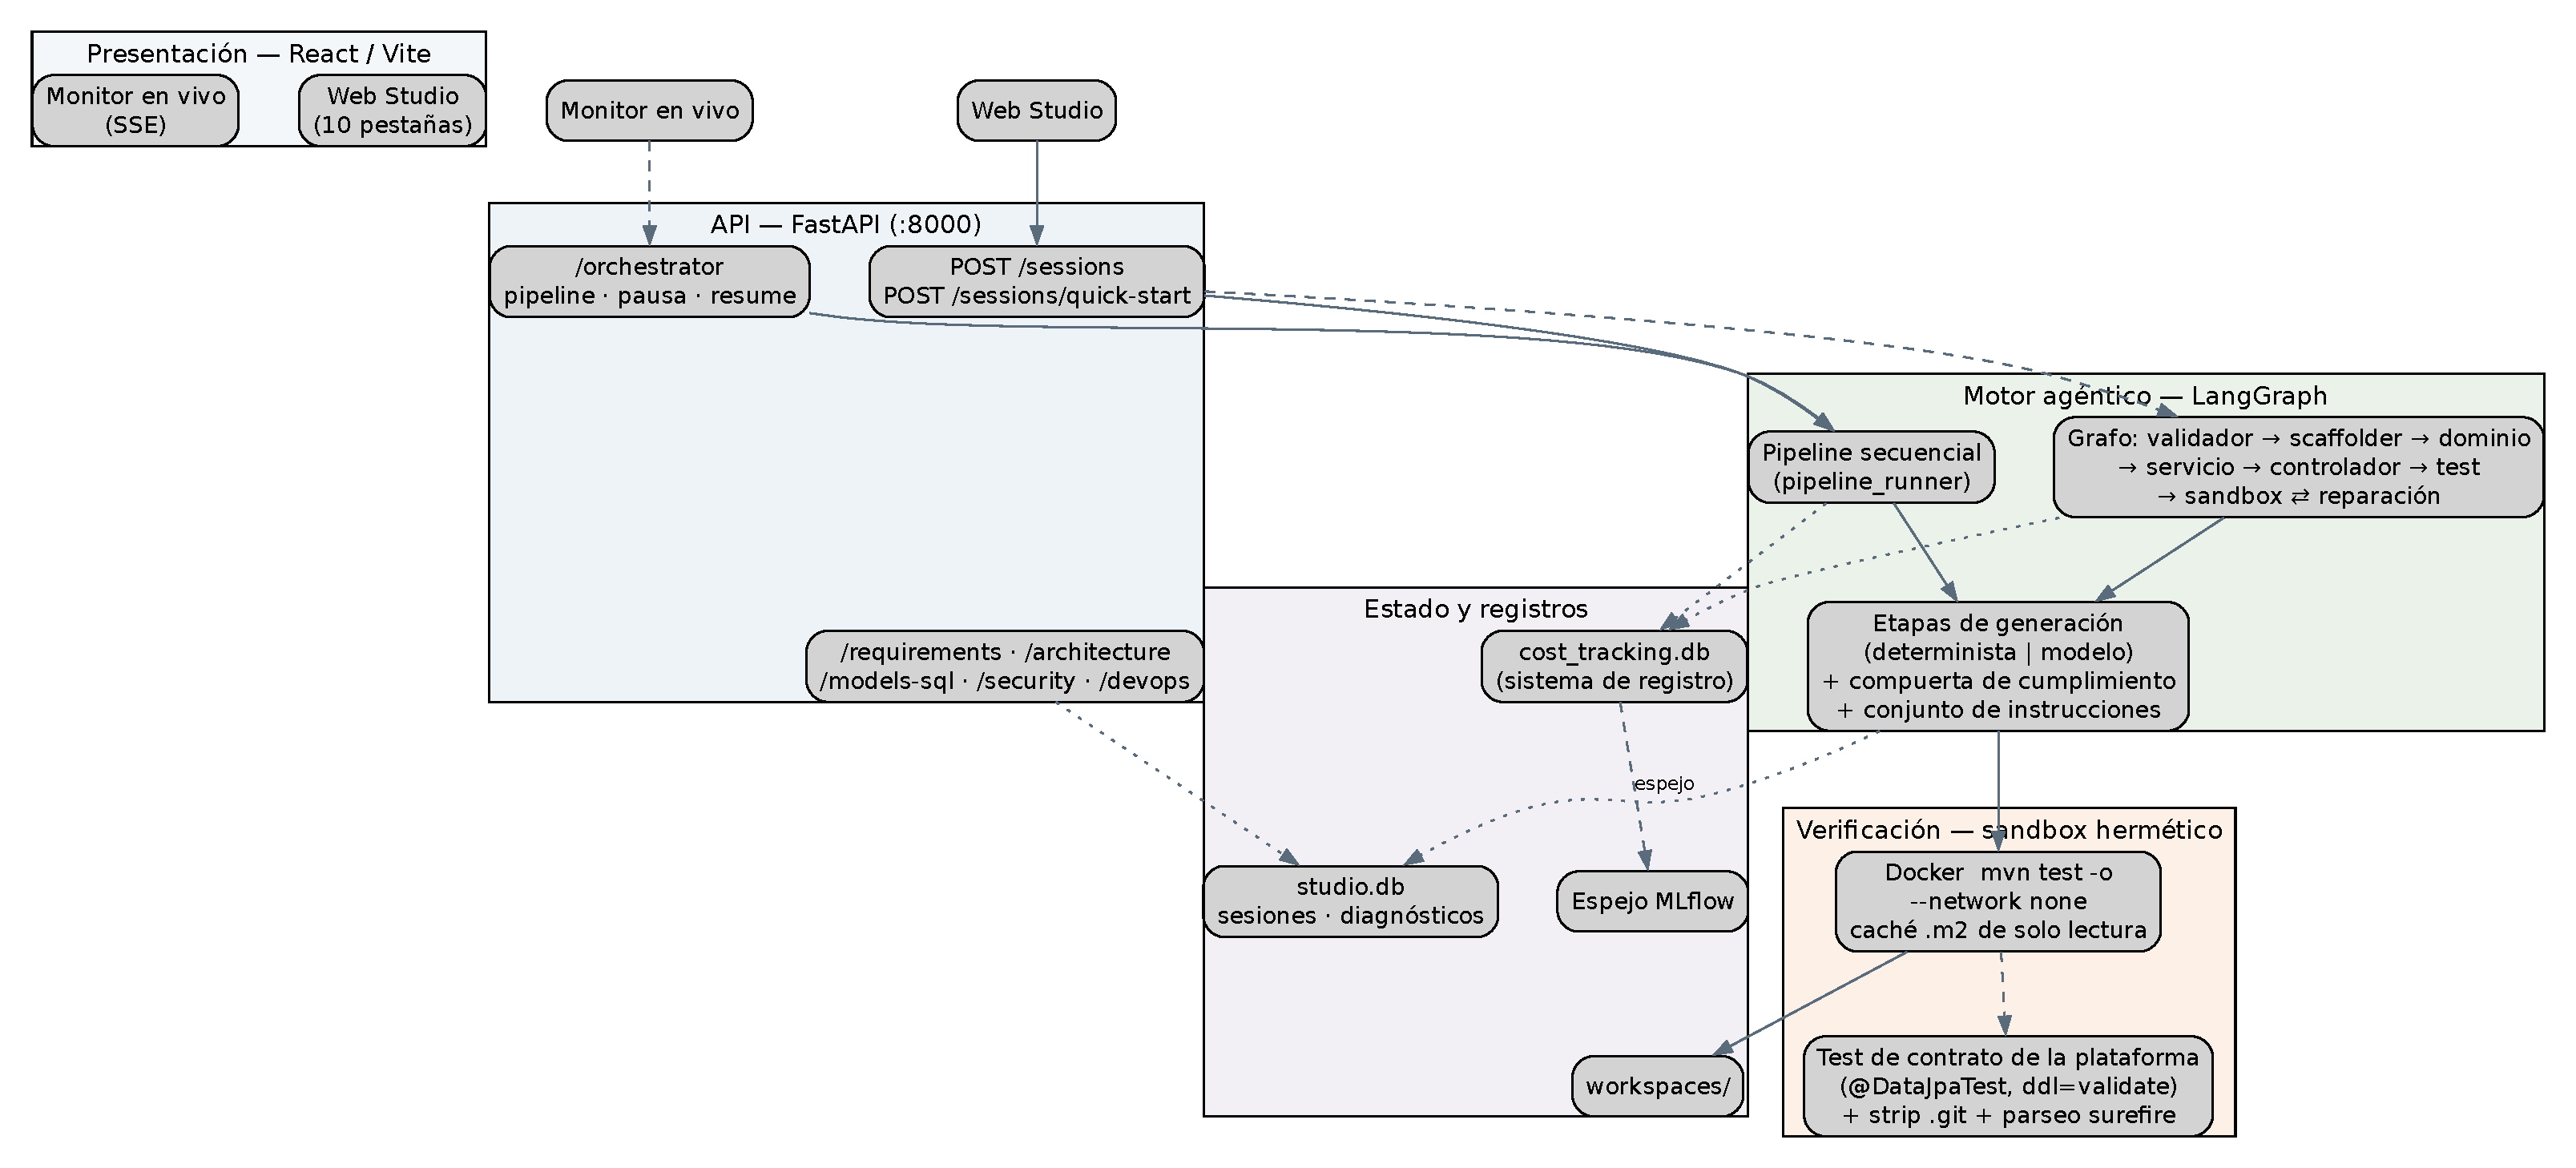
\includegraphics[width=\linewidth]{fig/architecture.pdf}
  \caption{Arquitectura del sistema: el estudio React sobre la API FastAPI, el motor
  agéntico LangGraph, el sandbox de verificación hermético y los almacenes de
  estado/coste.}
  \label{fig:architecture}
\end{figure}

\begin{figure}[htbp]
  \centering
  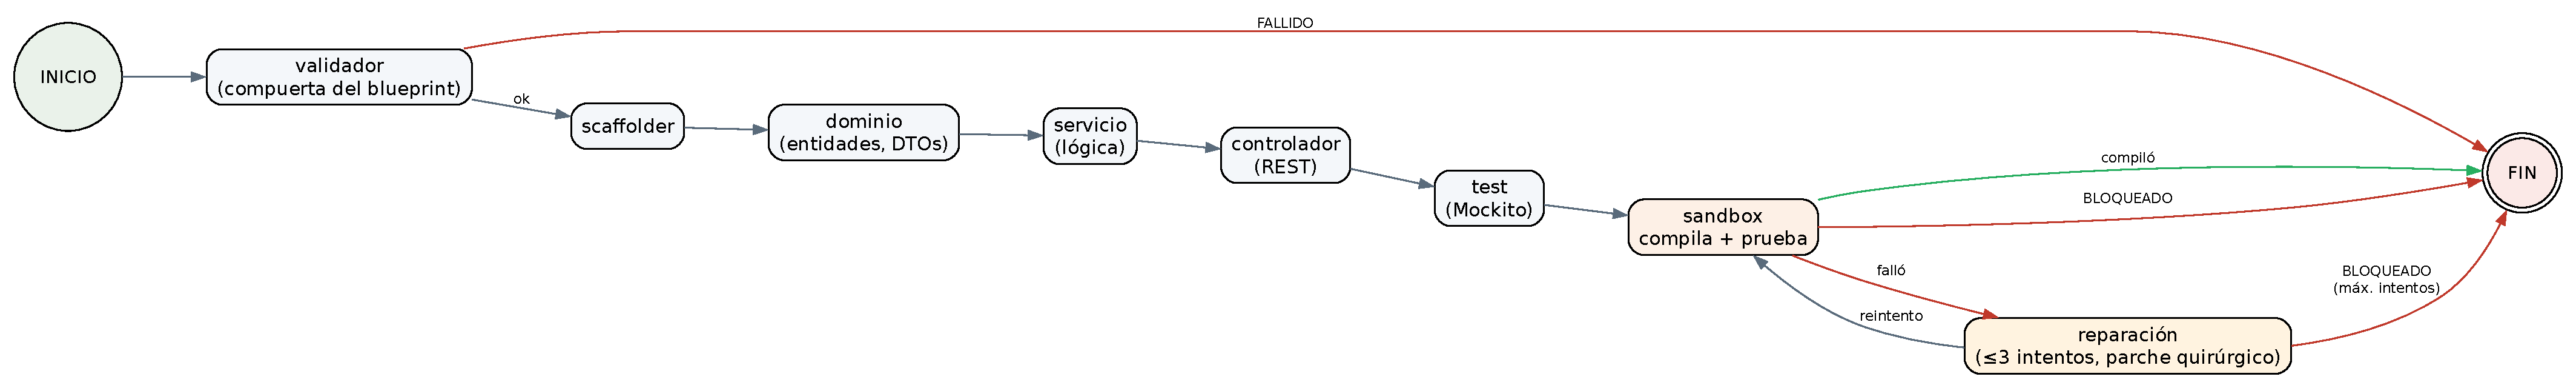
\includegraphics[width=0.82\linewidth]{fig/workflow.pdf}
  \caption{La máquina de estados de generación: una columna lineal con un ciclo
  acotado de reparación--sandbox.}
  \label{fig:workflow}
\end{figure}

\subsection{Inventario de servicios}

\begin{center}
\begin{longtable}{@{}p{0.34\textwidth}p{0.60\textwidth}@{}}
\toprule
\textbf{Servicio} & \textbf{Rol} \\
\midrule
\texttt{requirements\_service} & descomposición de historias BDD y síntesis de spec \\
\texttt{architecture\_service} & arquitectura en 4 capas y catálogo de componentes \\
\texttt{model\_sql\_service} & entidades JPA, DTOs, SQL de esquema/datos, diagrama ER \\
\texttt{test\_analysis\_service} & analizador estático de reglas constitucionales (familia A) \\
\texttt{security\_service} & SAST, secretos, conformidad de arquitectura (familia B) \\
\texttt{conformance\_diagnostics} & puntuador de conformidad determinista y atribuido por regla \\
\texttt{corpus\_report} & informe de medición por lote/corpus \\
\texttt{workspace\_verification} & eliminar VCS, inyectar test de contrato, ejecutar la compilación \\
\texttt{verification\_selection} & best-of-$k$: generar, verificar, detenerse en el primer éxito \\
\texttt{platform\_verification} & test de contrato de persistencia escrito por la plataforma \\
\texttt{skill\_contribution} & contribución por habilidad por leave-one-out \\
\texttt{llm\_factory} & detección de proveedor y construcción del cliente del modelo \\
\texttt{structured\_output} & salida del modelo restringida por esquema \\
\texttt{injection\_guard} & defensa contra prompt-injection del reflector \\
\texttt{queue\_service / lifecycle\_service} & concurrencia y orquestación de fases \\
\texttt{docker\_service / devops / export / git} & despliegue en contenedor, CI, ZIP, publicación \\
\texttt{registro de coste + espejo mlflow} & coste por llamada y por sesión, espejo \\
\bottomrule
\end{longtable}
\end{center}

\section{Resultados de verificación}
\label{sec:verification}

\subsection{Escalado de cobertura: la palanca de fiabilidad}

La selección guiada por verificación --- generar $k$ candidatos, verificar cada uno,
quedarse con el primero que pasa --- se mide aquí, no se toma prestada de otra clase de
tarea. El brazo de control del experimento de esta semana son 6 tareas, cada una
remuestreada 3--4 veces con las mismas instrucciones y modelo; la fórmula de cobertura
es $\mathrm{coverage}(k)=1-(1-p)^k$ (\emph{Large Language Monkeys},
\texttt{arXiv:2407.21787}).

\begin{center}
\begin{tabular}{@{}lrl@{}}
\toprule
\textbf{Métrica} & \textbf{Valor} & \\
\midrule
pass@1 (una muestra) & \textbf{78.3\%} & \\
cobertura $k{=}1$ & 83.3\% & \\
cobertura $k{=}2$ & 83.3\% & \\
cobertura $k{=}3$ & \textbf{100.0\%} & 6 de 6 tareas \\
cobertura $k{=}4$ & 100.0\% & \\
\bottomrule
\end{tabular}
\end{center}

A \$0.065 por servicio generado, tres candidatos cuestan \textbf{\$0.20 por servicio
fiable}. Advertencias, declaradas y no suavizadas: $n{=}6$ tareas, un modelo, un
proveedor; esto es una demostración de la palanca, no un benchmark, y la dirección
(la cobertura es monótona en $k$) es robusta mientras que el 100\% es ``6 de 6
tareas''.

\subsection{El verificador es intermitentemente inestable}

El mismo espacio de trabajo congelado, recompilado bajo carga antes, pasó 4 de 6
veces; recompilado secuencialmente, dos espacios de trabajo pasaron 8 de 8 cada uno.
El fallo, cuando ocurre, es una \texttt{PluginContainerException} de surefire sobre un
import foráneo de \texttt{surefire-shared-utils} --- \emph{después} de que todos los
tests hayan pasado.

La inestabilidad no es, por tanto, un defecto de código por espacio de trabajo. Es
intermitente y correlacionada con la carga, y la hipótesis principal es la
configuración de montaje: \texttt{DOCKER\_MOUNT\_SUFFIX=:Z} es un reetiquetado SELinux
\emph{privado}, correcto para un espacio de trabajo por sesión pero incorrecto para
una \emph{caché Maven compartida de solo lectura} montada por muchos contenedores
concurrentes. Dos contenedores reetiquetando una fuente compartida con \texttt{:Z} es
una causa conocida de exactamente esta clase de fallo intermitente de realm de clases.
La corrección propuesta es aplicar \texttt{:Z} solo al espacio de trabajo y dejar la
caché sin reetiquetar (o \texttt{:z}), confirmada por una compuerta de repetibilidad.

\begin{notebox}[colframe=warn]
\textbf{Por qué esto condiciona todo lo posterior.} Un verificador que se voltea
$\approx$33\% de las ejecuciones no puede servir como oráculo de admisión: la
cobertura prometería de más, una compuerta de admisión promovería ruido, y el teorema
de Ratchet (\texttt{arXiv:2605.22148}) dice que un juez tan ruidoso no retira nada a
ningún tamaño de muestra. Hacer el oráculo determinista es, por tanto, el prerrequisito
de toda medición posterior --- incluido el bucle de optimización de habilidades, que
permanece cerrado tras él.
\end{notebox}

\section{Coste y uso}
\label{sec:cost}

Los costes se registran por llamada y por sesión en el almacén SQLite local
(\texttt{backend/cost\_tracking.db}), que es el \textbf{sistema de registro}, y se
espejan en MLflow (\texttt{mlflow.db}). Ambos se comparan aquí, no se fusionan.

\subsection{Sistema de registro (autoritativo)}

\begin{center}
\begin{tabular}{@{}lrrr@{}}
\toprule
\textbf{Alcance} & \textbf{Llamadas} & \textbf{Coste (USD)} & \textbf{Tokens salida} \\
\midrule
Experimento de polaridad (\texttt{p4}) & 750 & \textbf{6.58} & --- \\
Línea base cinco congelados (\texttt{corpus}) & 120 & 0.63 & --- \\
Diez difíciles & 50 & 0.64 & --- \\
Sondas / sesiones sueltas & $\approx$250 & $\approx$0.16 & --- \\
\midrule
\textbf{Total} & \textbf{1172} & \textbf{8.01} & \textbf{12.28M} \\
\bottomrule
\end{tabular}
\end{center}

Las 1172 llamadas fueron \texttt{deepseek-flash}. Total de tokens de entrada 6.45M,
de salida 12.28M. El coste dominante es el experimento de polaridad de instrucciones,
que es una medición terminada (un nulo), no un drenaje continuo.

\subsection{Espejo MLflow (y dónde se ha desviado)}

\begin{center}
\begin{tabular}{@{}lrrrr@{}}
\toprule
\textbf{Experimento} & \textbf{Runs} & \textbf{Coste (USD)} & \textbf{Tok entr.} & \textbf{Tok sal.} \\
\midrule
\texttt{Default} (legado) & 877 & 5.41 & 4.63M & 8.20M \\
\texttt{agentia} (actual) & 114 & 0.98 & 0.78M & 1.52M \\
\midrule
\textbf{Total espejo} & 991 & \textbf{6.39} & 5.40M & 9.72M \\
\bottomrule
\end{tabular}
\end{center}

\begin{notebox}[colframe=warn]
\textbf{El espejo se ha desviado.} MLflow totaliza \textbf{\$6.39} frente a los
\textbf{\$8.01} del sistema de registro --- una subestimación de $\approx$\$1.62
(20\%), con $\approx$181 llamadas menos y totales de tokens que también discrepan. El
espejo está dividido entre un experimento legado y uno actual, y solo se escriben
métricas por llamada (faltan los agregados de sesión). La afirmación anterior de que
``el espejo funciona y coincide'' ya no es cierta para los datos actuales. Hasta que
se repare el sink, el almacén local es la única cifra a citar, y un informe de coste
generado solo desde MLflow subestimaría el gasto.
\end{notebox}

\section{Hallazgos y próximos pasos}
\label{sec:findings}

\begin{enumerate}[leftmargin=1.4em]
  \item \textbf{Hacer determinista el verificador antes de gastar más.} Separar el
  sufijo de montaje (espacio de trabajo \texttt{:Z}, caché compartida sin
  reetiquetar) y añadir una compuerta de repetibilidad: un espacio de trabajo
  congelado debe recompilar $N/N$ veces.
  \item \textbf{Hacer que la medida pueda moverse.} El instrumento de conformidad lee
  0 en compilaciones que fallan; exponer las clases de fallo del analizador de
  reparación como hallazgos acumulados para que un fallo de compilación sea
  atribuible.
  \item \textbf{Usar la selección guiada por verificación como mecanismo de fiabilidad
  ya.} Está medida (\$0.20/servicio a $k{=}3$), no necesita entrenamiento y es la
  palanca que la literatura sitúa en primer lugar.
  \item \textbf{Reparar el espejo de coste.} El espejado a nivel de sesión no se está
  poblando; restaurarlo o la UI de MLflow subestima el gasto.
  \item \textbf{Resolver la inconsistencia del límite de reparación} (constitución 3
  vs \texttt{config.py} 5).
  \item \textbf{Dejar cerrado el bucle de optimización de habilidades} hasta que los
  puntos 1 y 2 pasen sus compuertas; el experimento de polaridad de instrucciones que
  era su entrada más prometedora es un nulo (prohibición vs control: 1 victoria, 3
  derrotas, 2 empates).
\end{enumerate}

\end{document}
